\chapter{Theoretical background}

This chapter explores three key concepts that power the learning platform: spaced repetition algorithm, Large Language Models and the REST (REpresentational State Transfer). Spaced repetition is a learning technique, that can help improve long-term retention by scheduling the learning material with increasing intervals. It is an evidence-based technique and is usually performed with flashcard-like methods, which makes it practical to implement into the learning platform. On the other hand, LLMs act as knowledge bases that generate targeted questions.

REST is an architectural style for distributed hypermedia systems, originally introduced by Roy Fielding \cite{fielding2000} in his 2000 doctoral dissertation. Despite its widespread adoption in modern web development, it is worth exploring in detail here, particularly focusing on HATEOAS (Hypermedia as the Engine of Application State) - a less commonly understood principle that forms a crucial foundation for a concept discussed later in this thesis. By combining these techniques, the platform can create a tailored learning experience.

\section{Spaced Repetition}
TODO - everything about the algorithm, how does it work, examples, implementation
TODO - mention the algorithm is not an exact algorithm with concrete parameters and constants, but more like a guideline
TODO - TODO mention my algo, show a pseudo code, and mention this needs a lot of feedback from real users to 

\section{Large Language Models}
TODO - What is a large language model, how do they work briefly, supervised finetuning, qlora, prompt engineering, dataset, wikipedia articles, the final model(s), how we integrated it to the platform. This is mostly Máté's topic so when he is done i will start to write this part

\section{REST}

The REST architectural style has six guiding principles, all of which must be satisfied by a REST-ful service. Roy names them \cite[Chapter 5]{fielding2000}: Client-Server, Stateless, Cache, Uniform interface, Layered system, and Code-On-Demand.

\subsection{Client-Server}

The Client-Server is the most fundamental architectural style in network-based applications. It consists of two primary components: clients and servers, each with distinct responsibilities, as illustrated in Figure ~\ref{fig:client-server}.

\begin{figure}[!h]
\centering
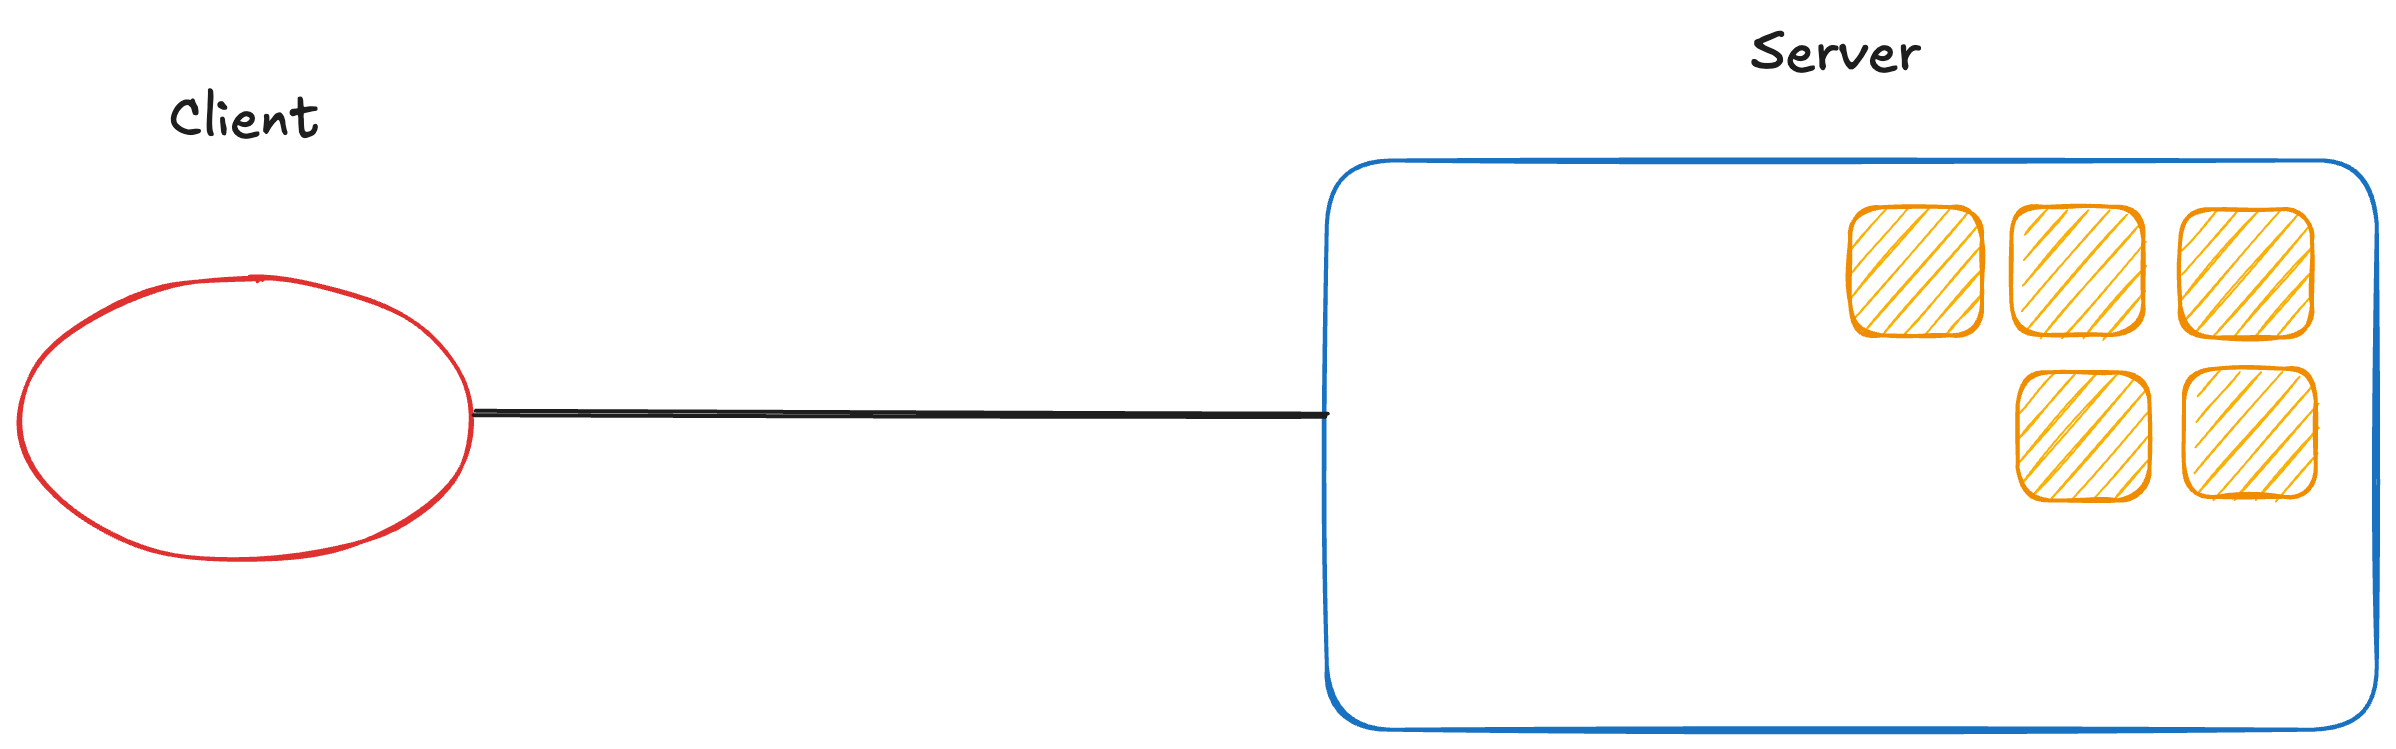
\includegraphics[width=0.8\textwidth, keepaspectratio]{figures/client-server.png}
\caption{Client-Server architectural style (own visualization inspired by Fielding \cite{fielding2000})}
\label{fig:client-server}
\end{figure}

In this architecture, clients initiate requests to servers, which manage resources. The server listens for incoming requests and either processes them by providing the requested resource or service or rejects them if they cannot be fulfilled. This separation of concerns allows client and server components to evolve independently \cite{sinha1992}.

\subsection{Client-Stateless-Server}

This principle requires that all communication between the parties be stateless, as illustrated in Figure ~\ref{fig:stateless}. This means that each request from the client must contain all the information necessary for the server to understand and process it\cite{MESBAH20082194}. As a result, the session state must be stored entirely on the client side.\cite[Section 3.4.1.]{fielding2000}

\begin{figure}[!h]
\centering
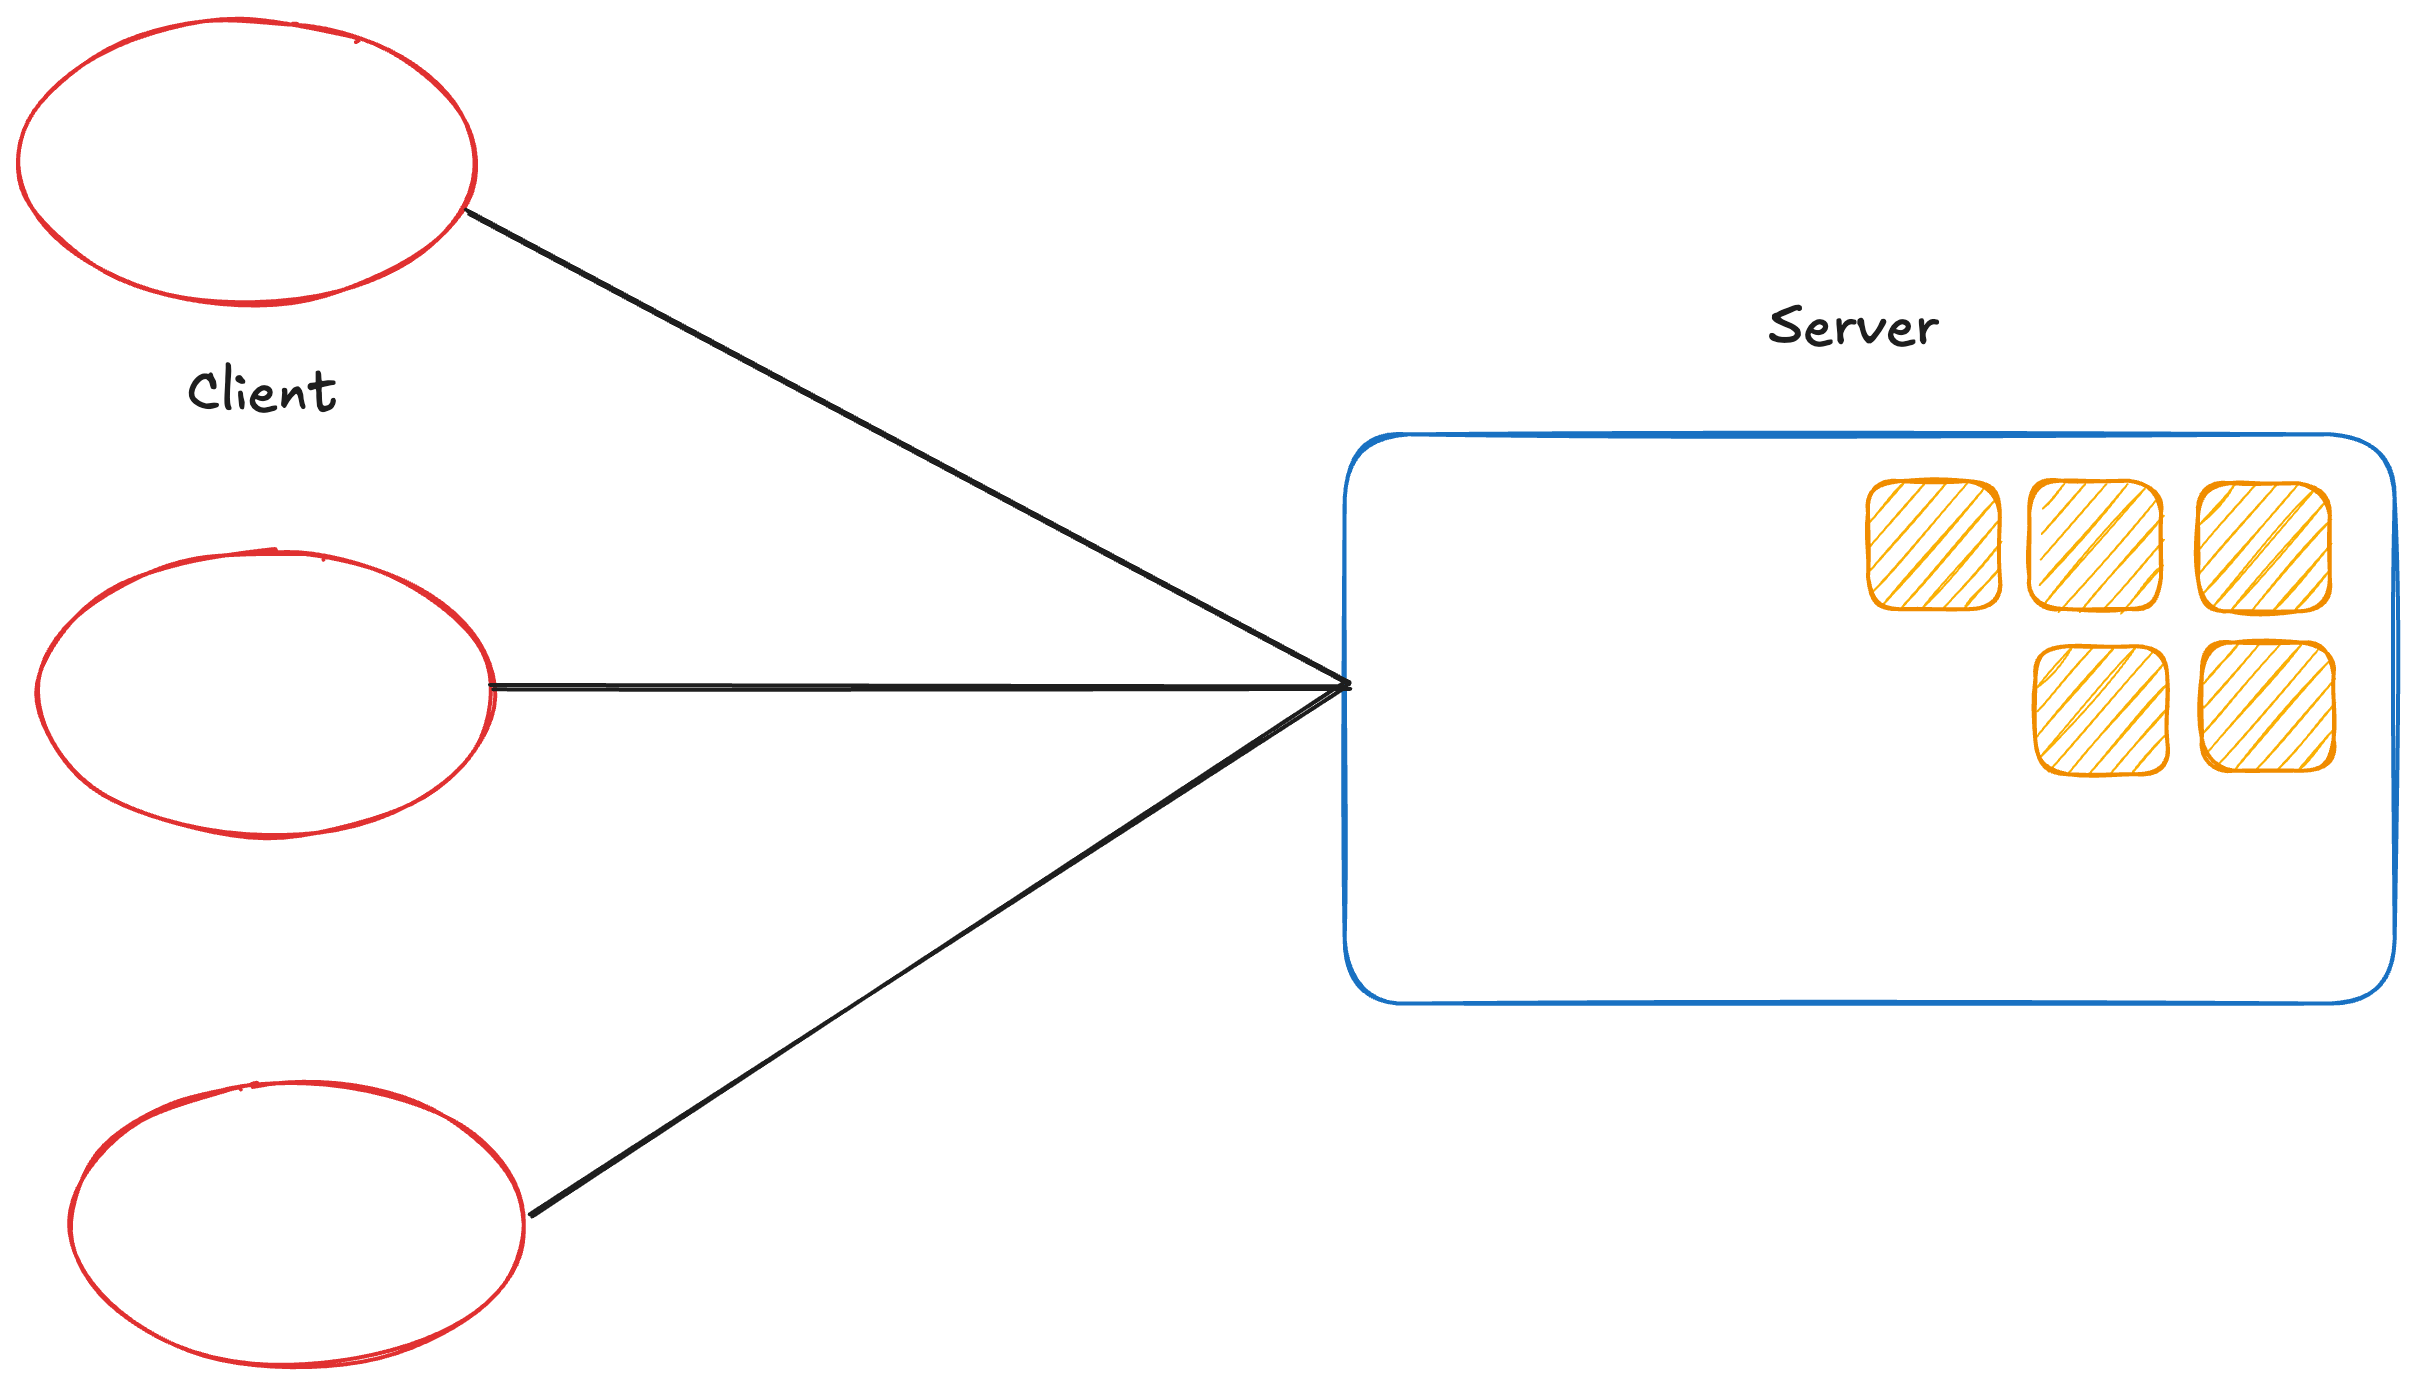
\includegraphics[width=0.8\textwidth, keepaspectratio]{figures/stateless.png}
\caption{Client-Stateless-Server (own visualization inspired by Fielding \cite{fielding2000})}
\label{fig:stateless}
\end{figure}

This constraint improves visibility, reliability, and scalability. However, it can decrease network performance due to the overhead of sending complete state information with each request \cite[Section 5.1.3]{fielding2000}.

\subsection{Cache}

The cacheable constraint requires that the response be labeled cacheable or non-cacheable. When labeled cacheable, the client has the right to use data later for a specified period.

\begin{figure}[!h]
\centering
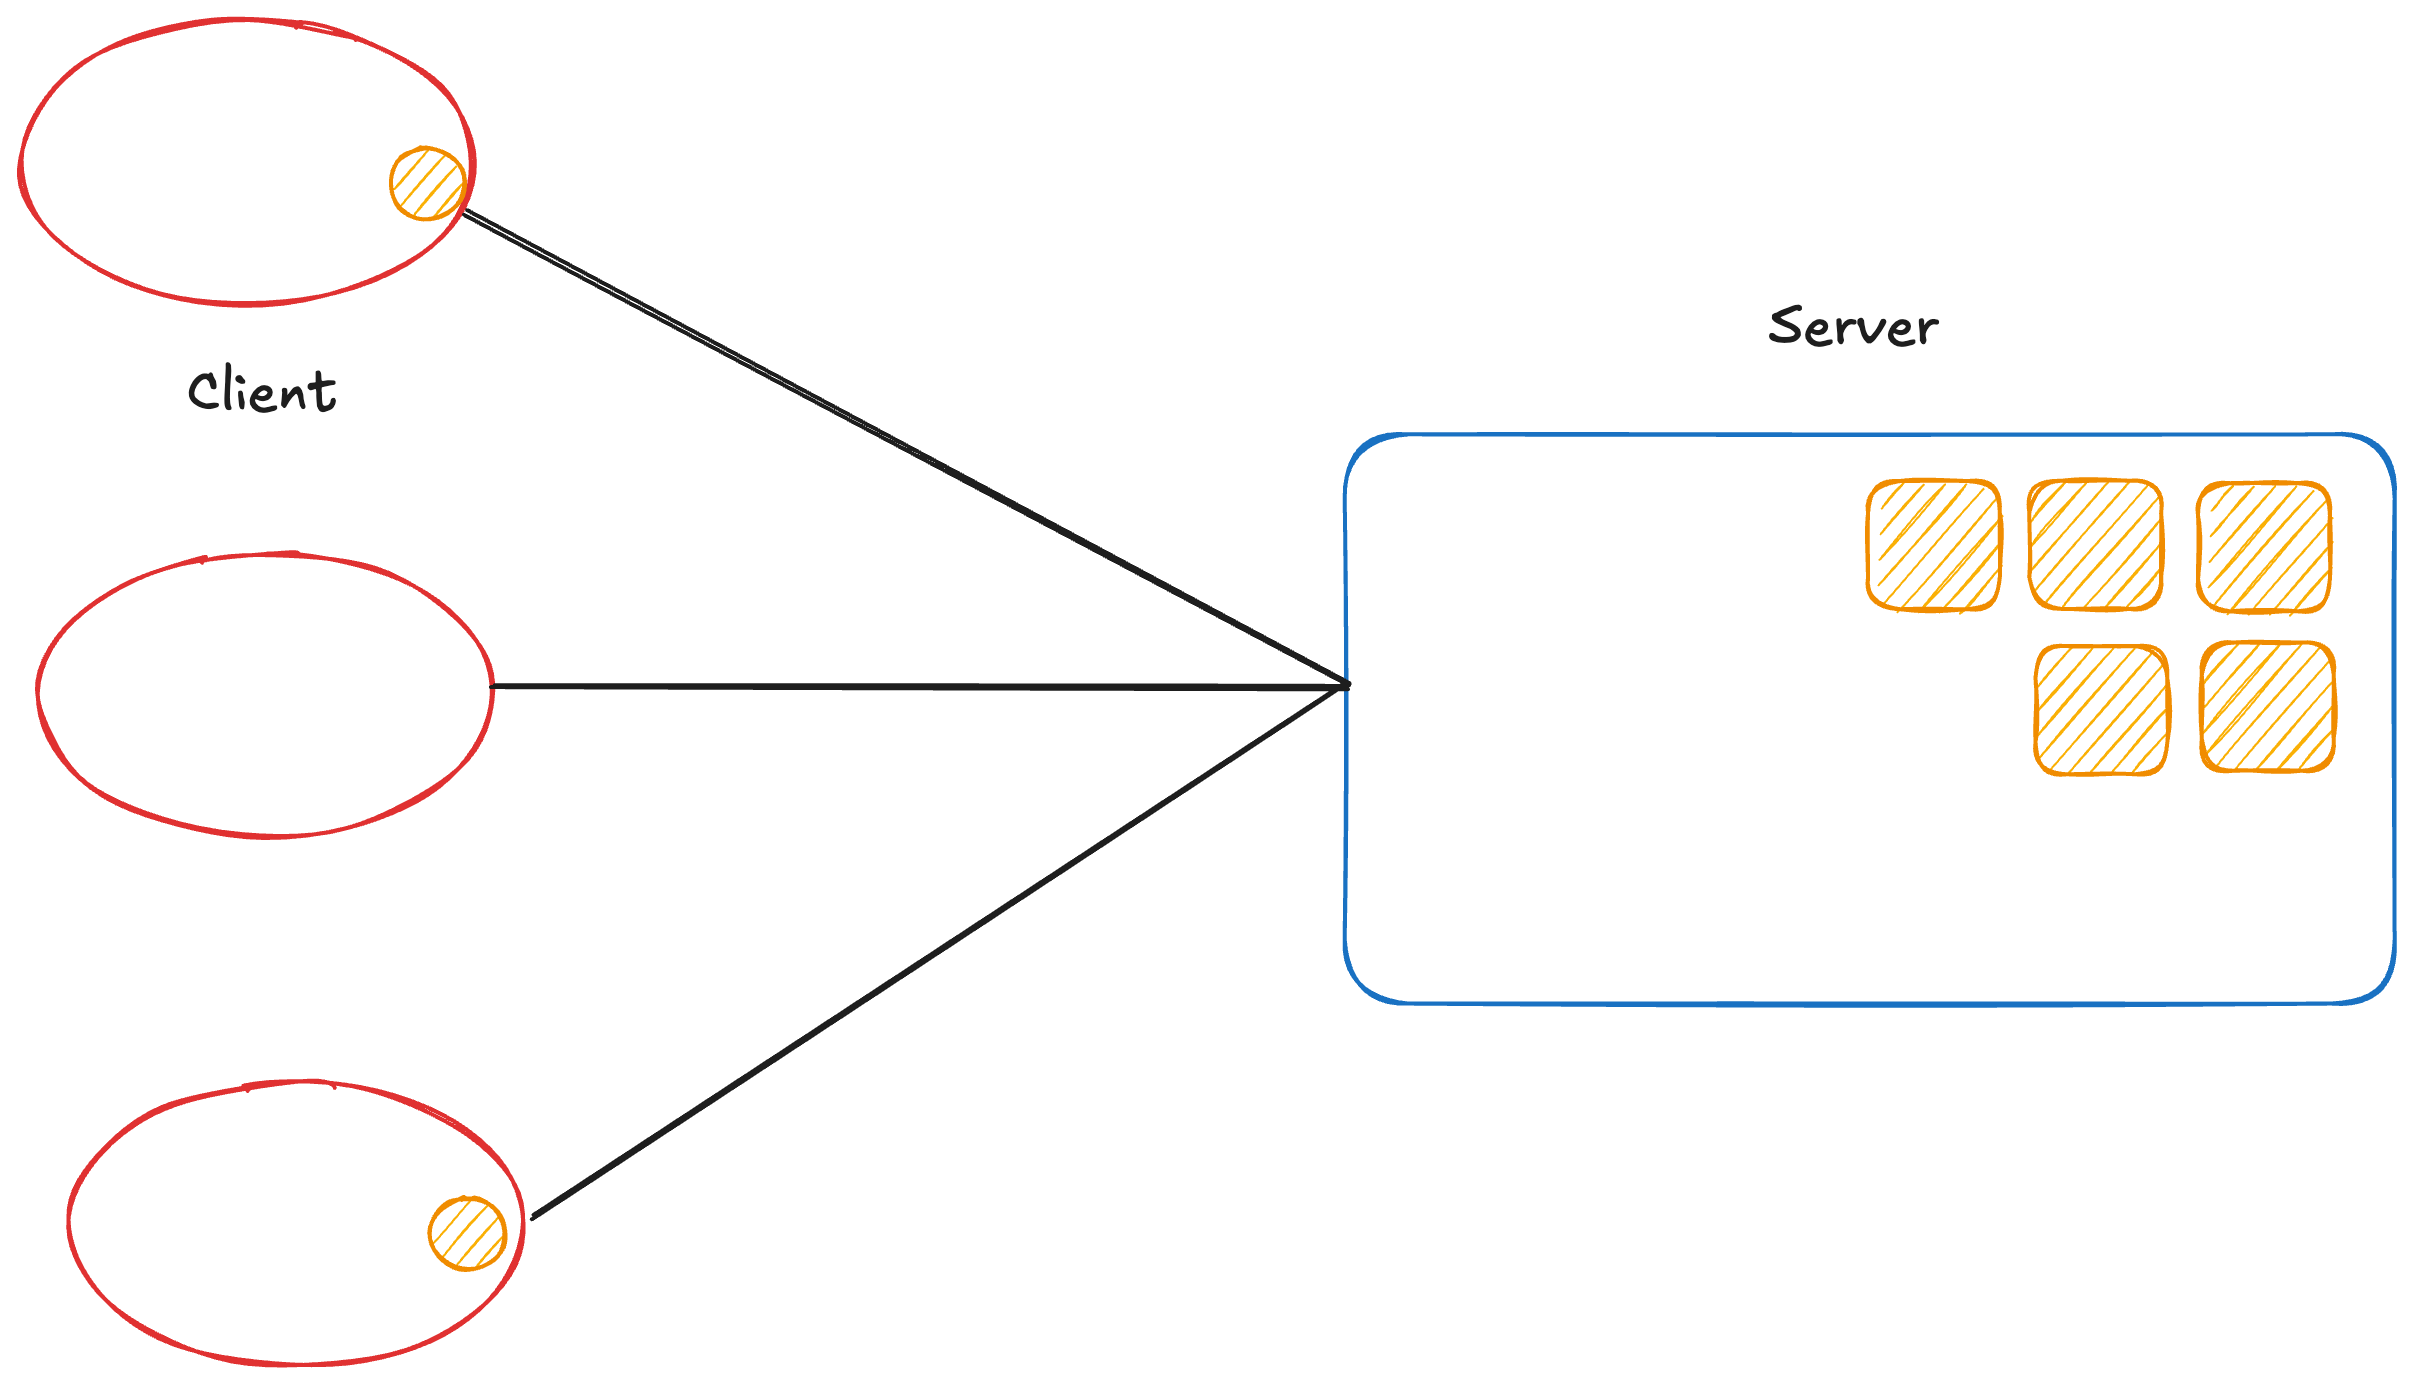
\includegraphics[width=0.8\textwidth, keepaspectratio]{figures/cache.png}
\caption{Cache (own visualization inspired by Fielding \cite{fielding2000})}
\label{fig:cache}
\end{figure}

\subsection{Uniform interface}
This principle says the REST services should ensure uniformity through these interface constraints:

\begin{itemize}
\item \textbf{Resource identification}: Each resource must be identified by a unique identifier URI. In practice, this is implemented by using URLs as identifiers.
\item \textbf{Resource manipulation}: Each resource should have a uniform representation on the server that the client can use to modify them.
\item \textbf{Self-descreptive messages}: Each request should contain enough information for the server to describe how to process them.
\item \textbf{HATEOAS}: The client application should dynamically drive all other resources and interactions using hyperlinks.
\end{itemize}

\begin{figure}[!h]
\centering
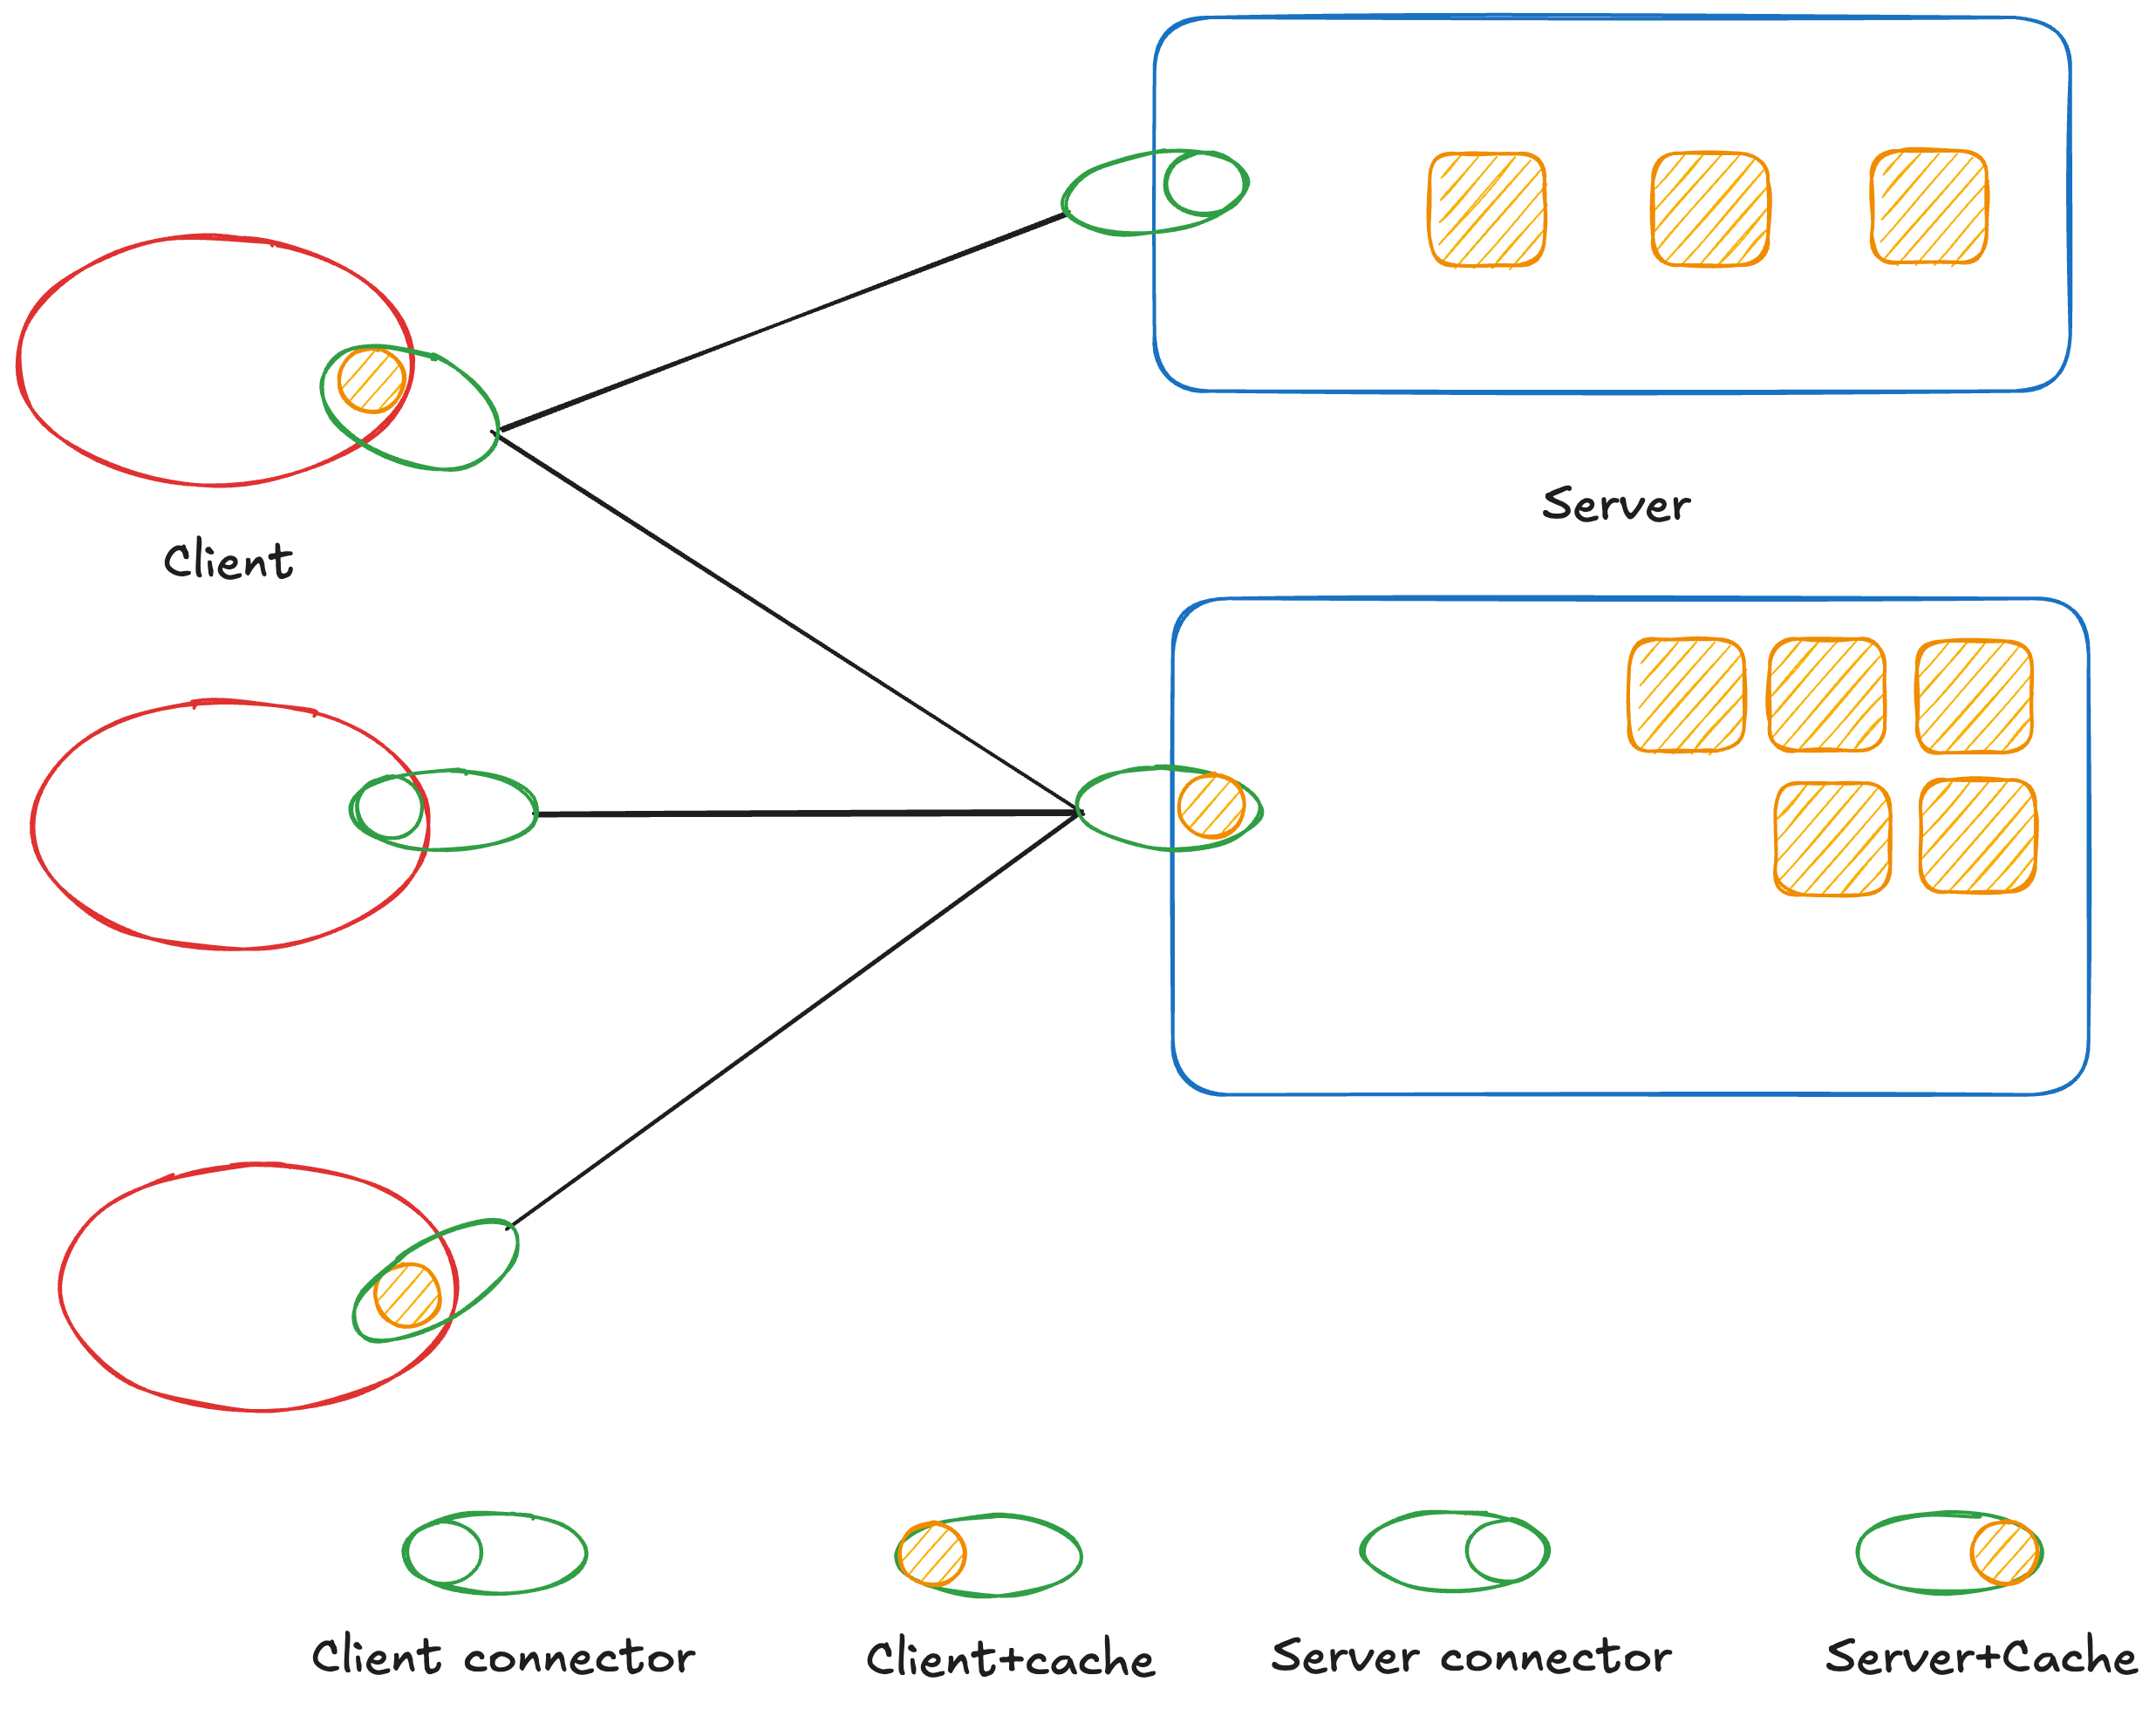
\includegraphics[width=0.8\textwidth, keepaspectratio]{figures/uniform-interface.png}
\caption{Uniform interface (own visualization inspired by Fielding \cite{fielding2000})}
\label{fig:uniform-interface}
\end{figure}

\subsubsection{HATEOAS}

HATEOAS is a small constraint that many people tend to forget. If we take the constraint strictly, most REST applications would not be REST applications. This is usually fine because most applications work differently than Fielding imagined in his dissertation back in the day. If we, a service, comply with it, all of its responses should contain the accessed data and the available actions as hyperlinks. The listing \ref{lst:hateoas} shows an example of a compliant response.

\begin{lstlisting}[caption=An HATEOAS response in JSON format,label=lst:hateoas, float]
{
  "accountId": "123456789",
  "accountName": "John Doe",
  "balance": 1500,
  "links": [
    {
      "rel": "self",
      "href": "http://examplebank.com/accounts/123456789",
      "method": "GET"
    },
    {
      "rel": "deposit",
      "href": "href": "http://examplebank.com/accounts/123456789/deposit",
      "method": "POST"
    },
    {
      "rel": "withdraw",
      "href": "href": "http://examplebank.com/accounts/withdraw",
      "method": "POST"
    }
  ]
}
\end{lstlisting}

One of the main ideas of HTMX is to be HATEOAS compliant. The website pages are generated dynamically on the server to contain the requested resource and all the actions available for the given resource. The server generates the page and adds HTMX requests to desired elements representing the actions.

\subsection{Layered System}

A layered system is another architectural style that allows splitting the service into different components placed in other layers. It will enable grouping, hiding, and defining behaviors between them. "Layers can be used to encapsulate legacy services and to protect new services from legacy clients" \cite{fielding2000}. These layers can also improve system scalability by enabling load balancing of the services. "The primary disadvantage of layered systems is that they add overhead and latency to the processing of data, reducing user-perceived performance" \cite{Clark1990ArchitecturalCF}. Figure \ref{fig:layered-system} shows the architecture of a complex, layered system.

\begin{figure}[!h]
\centering
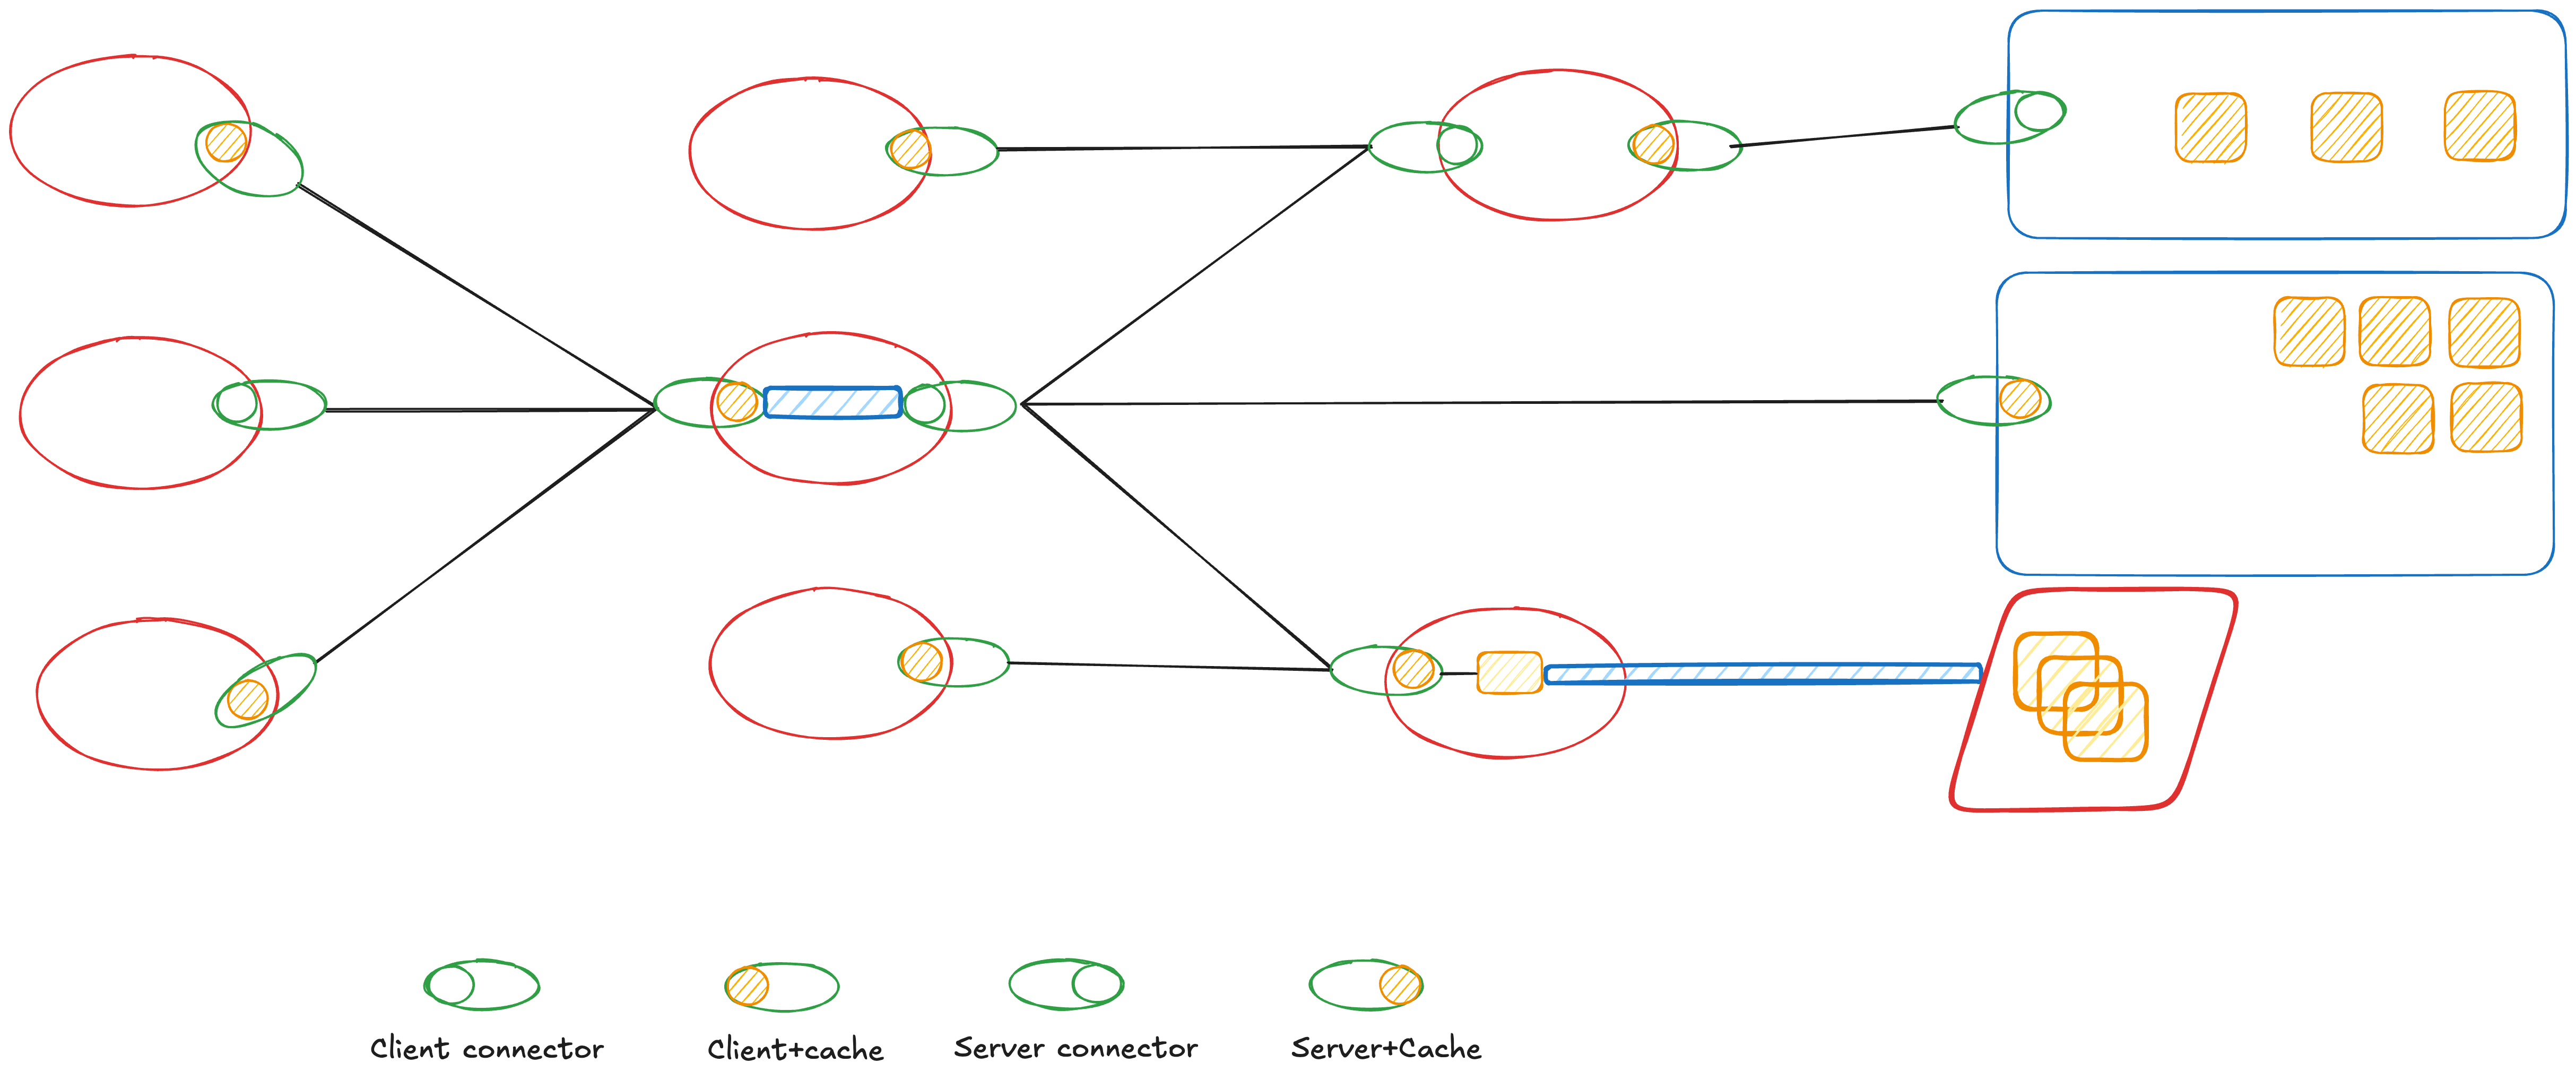
\includegraphics[width=0.8\textwidth, keepaspectratio]{figures/layered-system.png}
\caption{Layered System (own visualization inspired by Fielding \cite{fielding2000})}
\label{fig:layered-system}
\end{figure}

\subsection{Code-On-Demand}

Code-On-Demand is an optional constraint that the figure \ref{fig:code-on-demand} shows. It allows a client to extend its functionality by downloading and executing code as a script from a different source. "This simplifies clients by reducing the number of features required to be pre-implemented" \cite{fielding2000}. However, it is only an optional constraint because it reduces the overall visibility of a service.
 
\begin{figure}[!h]
\centering
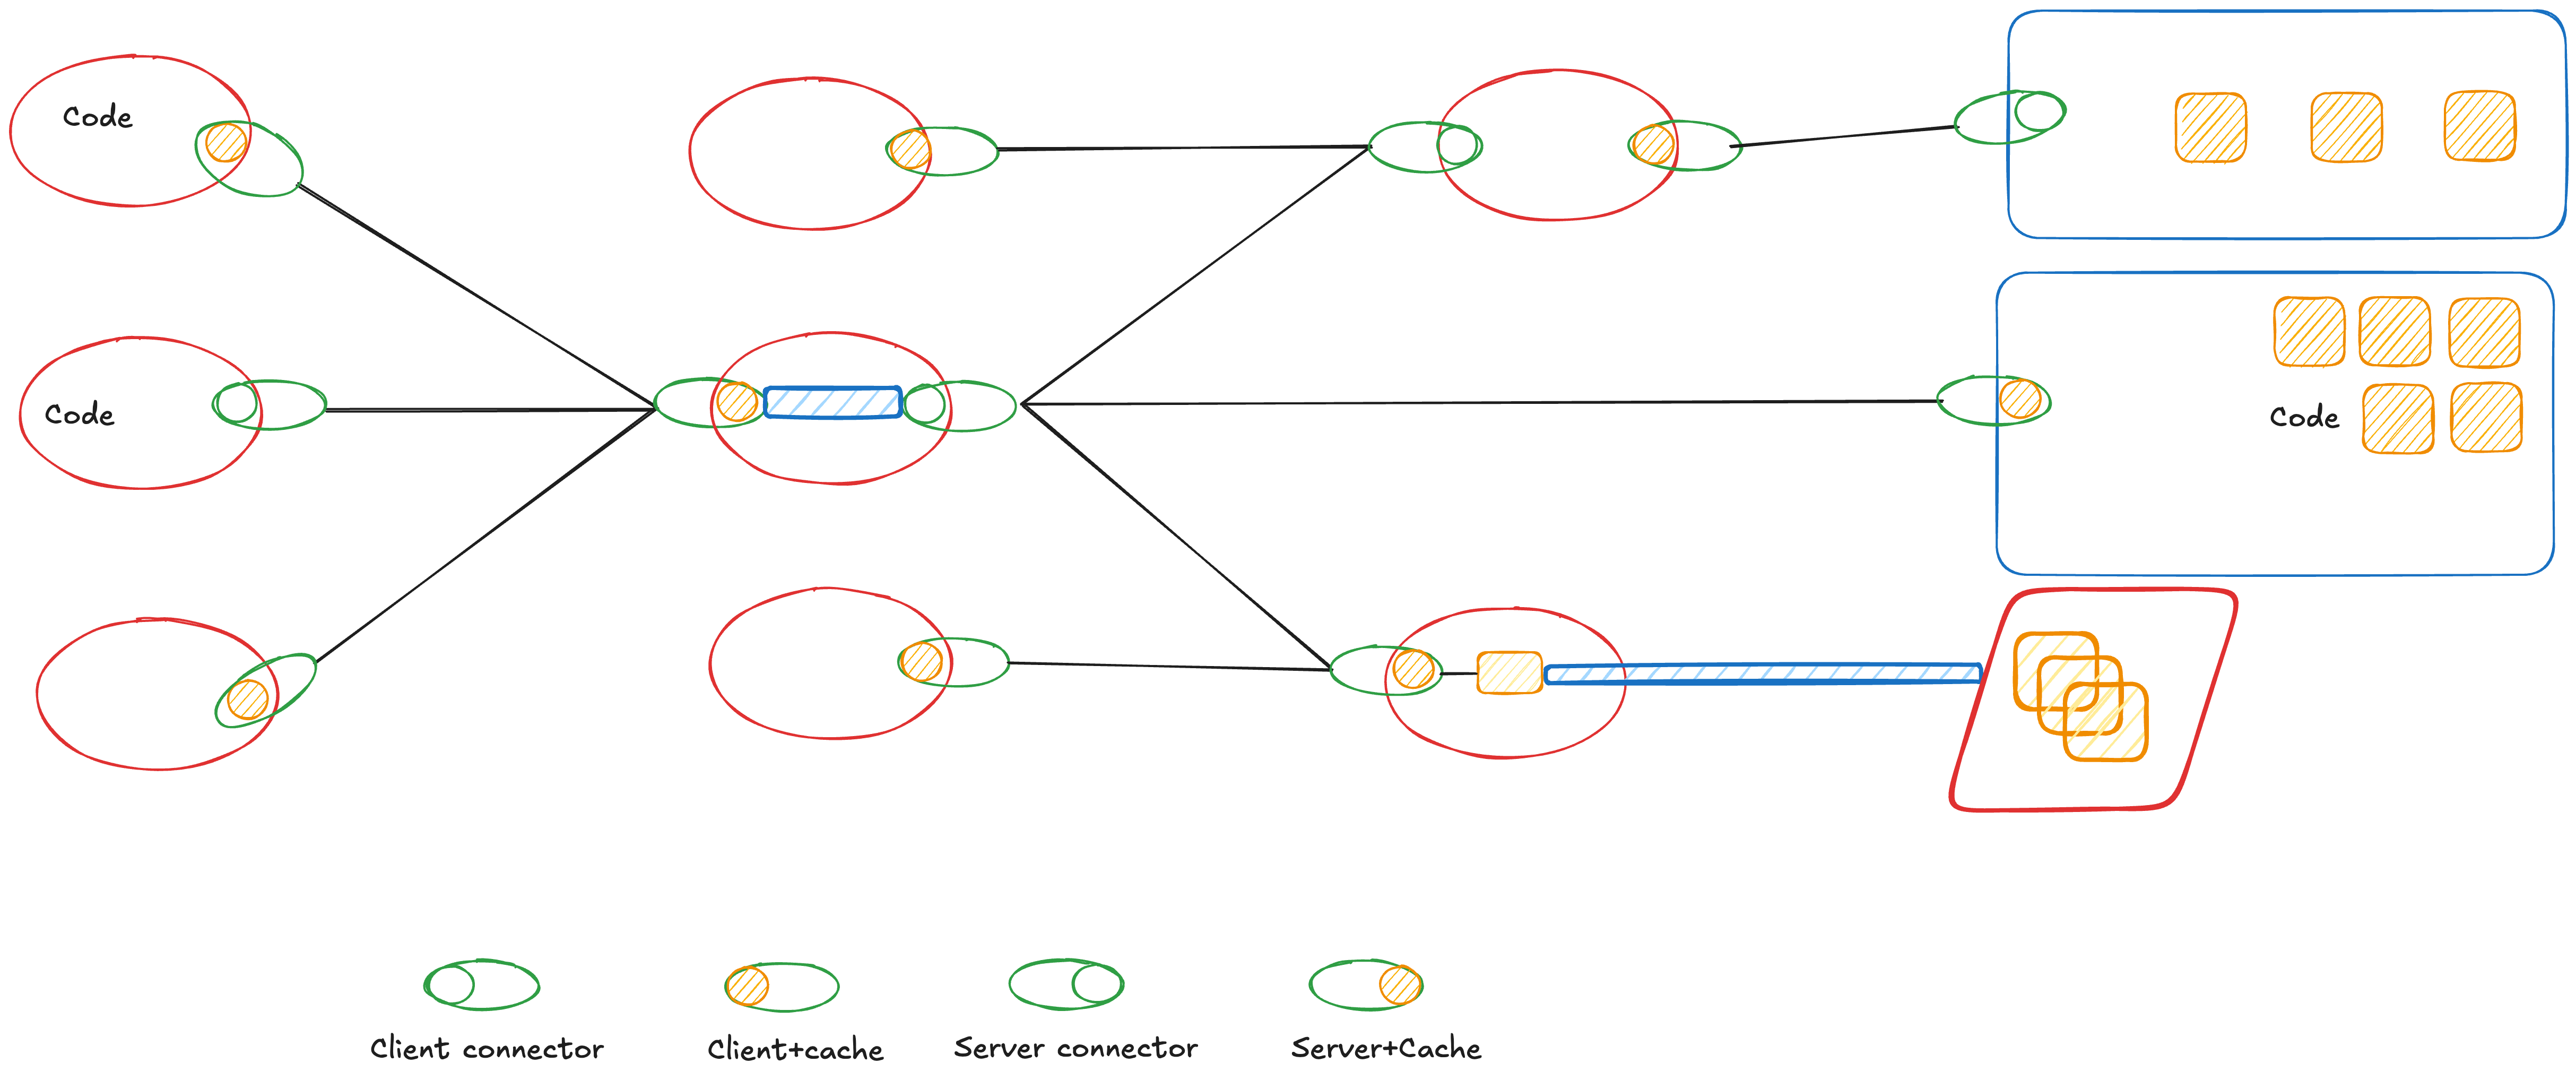
\includegraphics[width=0.8\textwidth, keepaspectratio]{figures/code-on-demand.png}
\caption{Code-On-Demand (own visualization inspired by Fielding \cite{fielding2000})}
\label{fig:code-on-demand}
\end{figure}